\documentclass[8pt, letterpaper]{article}
\usepackage[utf8x]{inputenc}
\usepackage[russian]{babel}
\usepackage{graphicx}
\graphicspath{{pictures/}}
\usepackage{multicol}
\usepackage[margin=0.5in]{geometry}
\usepackage{fancyhdr} 
\usepackage{mathtools}

\fancypagestyle{firststyle}
{
\fancyfootoffset[R]{-12cm} 
\fancyhead[C]{ОТВЕТЫ, УКАЗАНИЯ, РЕШЕНИЯ}
\renewcommand{\footrulewidth}{0.0 mm} 
\renewcommand{\headrulewidth}{0.0 mm}
\setlength{\headheight}{80pt}
\fancyfoot[R]{\thepage}
}
\newenvironment{myfont}{\fontfamily{phv}\selectfont}{\par}
\begin{document}
\begin{titlepage}
	\newpage
	\begin{center}
		{\bfseries Национальная научно-образовательная корпорация ИТМО
}
		
		Факультет ПИиКТ
		\vspace{6em}
		
		Лабораторная работа №6 \\
		
		
	\end{center}
	
	
	
	\begin{center}
		\Large Работа с системой компьютерной вёрстки \LaTeX \linebreak
	\end{center}
	
	\begin{center}
		Вариант №119
	\end{center}
	\vspace{\fill}
	
	
	\noindent Работу выполнила: Кононова Виктория Владимировна, P3111 \\
	Преподаватель: Малышева Татьяна Алексеевна
	
	\vspace{3em}
	
	
	
	\begin{center}
		Санкт-Петербург 2022
	\end{center}
	
\end{titlepage}
\include{titlePageSLU}



\thispagestyle{firststyle}


\setlength{\columnsep}{0.5cm}
\setlength\parindent{1pt}
\begin{multicols}{2}

\fontsize{10pt}{12pt}\selectfont

4. Нужно многократно использовать тот факт, что касательные,
проведенные из одной точки к окружности, равны. Пусть ок-
ружностн касаются отрезка AD в точках P и O, стороны ВС —
в точках М и N (рис.12). Из равенства отрезков общих внеш-
них касательных между точками касания и равенства касатель-
ных, проведенных из точек D н К, получим: КР=DQ,
КD=МN, а затем, используя равенство касательных, проведен-
ных източки А, получим 2АК=АР+АQ — МN=АВ+АС — ВС.

\centering
\begin{tabular}{ p{0.5\linewidth}p{0.4\linewidth}  }
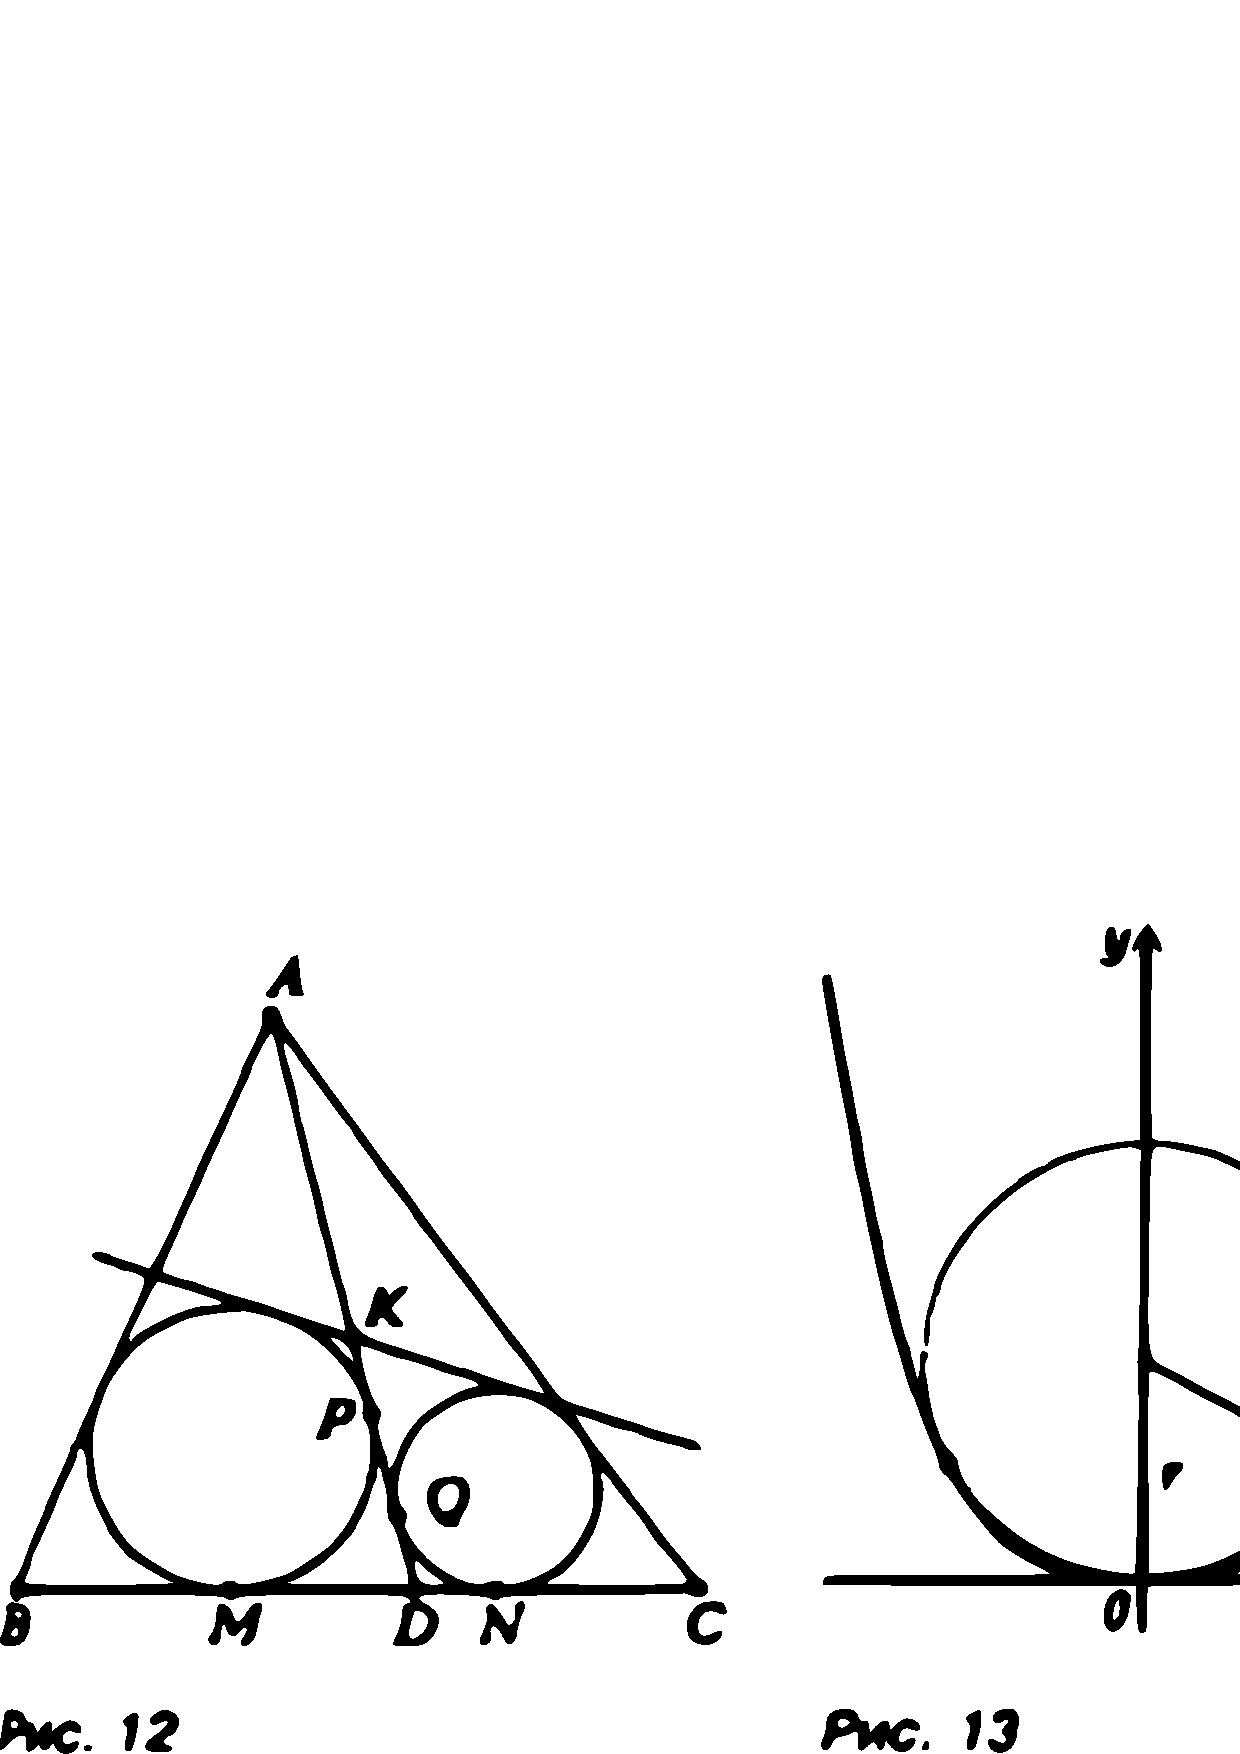
\includegraphics [width=0.5\linewidth]{Screenshot_1.png} & \includegraphics [width=0.5\linewidth]{Screenshot_3.png} \\
\setlength\parindent{20pt}
Рис. 12 & \setlength\parindent{13pt} Рис. 13
\end{tabular}
\flushleft
11 класс\\
1. Можно отрезать ст двух вершин тетраэдра (или от двух со-
седних вершии куба) два маленьких треугольника.
3. 32/4. Можно найти это значение г как максимальное, при
котором уравнения $y=x^4, x^2+(y-r)^2 =r^2$ имеют общее реше-
кие, отличное от $х=у=0$. А можно кроме этих двух уравнений
получить третье, используя тот факт, что для критического зна-
зения окружность имеет с графиком $y = x^4$ общие касательные
(в некоторой точке, отличной от х=у=0, см, рис. 13).

\textbf {\normalsize Избранные задачи Московской \\
 физической олимпиады}
\\
\vspace{5pt}
\hrule
\vspace{2pt}
Первый тур.\\
\vspace{1pt}
\hrule
\vspace{5pt}
9 класс

1. $v=\sqrt{\alpha/Mt}$. 2. Горки разъезжаются в противоположные сто-
рокы с почти одинаковыми скоростями $v=\sqrt{mgH/M}$.
3. $T_{1}^2/T_{2}^2=h_{1}/h_{2}$

10 класс\\
1. Брусок притягивается х стенке с силой $F = (2o^2l)/(pgd^2)$.
\columnbreak
\\
2. См. рис. 14: $R=\sqrt{L^2-g^2/w^4}$.
\flushleft
\includegraphics [width=0.4\textwidth]{Screenshot_2.png} \\ \centering Рис. 14
\label{fig:mpr}
\flushleft
3. Маятник движется по окружности в плоскости рисунка, имея энергию\\
$E=mgl+\frac{mu^2}{2}\phi(\frac{4gl}{v^2})$.\\
где $\phi(x)=0$, если $x$ - целое число, и $\phi(x)=1 - {x}$, если $x$ - нецелое, а {x} - его дробная часть.\\
11 класс\\
1. $(\frac{F_{1}}{F2})_{max} = \frac{16\pi^4l^2}{T^4g^2}$\\
2. Одно изображение ближе основного, а другое дальше от него на одно и то же расстояние l = 2d/n, где d - толщина стекла зеркала, а n - его показатель преломления.
\vspace{5pt}
\hrule
\vspace{-2pt}
Второй тур.\\
\vspace{7pt}
\hrule
\vspace{5pt}
9 класс\\
1. См. таблицу, в которой $t_{0} = 1$ c.
2. $w_{min} < w < w_{max}$, где\\
$w_{min} = \frac{\sqrt{g(\sqrt{h(2R-h)}-\mu(R-h))}}{\sqrt{h(2R-h)((R-h)+\mu\sqrt{h{2R-h)}}}}$ при $\mu < \frac{\sqrt{h(2R-h)}}{R-h}$
$w_{min} = 0$ при $\mu \geq \sqrt{h(2R-h)}/(R-h)$,
$w_{max} = \frac{\sqrt{g(\sqrt{h(2R-h)}+\mu(R-h))}}{\sqrt{h(2R-h)((R-h)-\mu\sqrt{h{2R-h)}}}}$ при $\mu < \frac{\sqrt{h(2R-h)}}{R-h}$ при $\mu < \frac{R-h}{\sqrt{h(2R-h)}}$,
$w_{max} = \infty$ при $\mu \geq (R-h)\sqrt{h(2R-h)}$.
\end{multicols}
\flushright
Таблица
\begin{tabular}{ |p{0.3\linewidth}| l | l | p{0.2\linewidth} | }

\hline

Возможный случай & При каких $s$ возможен & Начальная скорость & Путь, пройденный за вторую секунду \\ \hline

В течение двух секунд камень движется вверх & $s>\frac{3}{2}gt_{0}^2$ & $\frac{s}{t_{o}}+\frac{gt_{o}}{2}$ & $s-gt_{0}^2$ \\ \hline
Камень поворачивает в течение второй секунды & $\frac{gt_{0}^2}{2}<s<\frac{3}{2}gt_{0}^2$ & $\frac{s}{t_{0}}+\frac{gt_{0}}{2}$ & $\frac{5}{4}gt_{0}^2-2s+\frac{s^2}{gt_{0}^2}$ \\ \hline
Камень поворачивает в течение первой секунды & $\frac{gt_{0}^2}{4} < s < \frac{gt_{0}^2}{2}$ & $\frac{gt_{0}+\sqrt{4gs-g^2t_{0}^2}}{2}$ & $\frac{2gt_{0}^2-\sqrt{4gst_{0}^2-g^2t_{0}^4}}{2}$ \\ \hline
Камень поворачивает в течение первой секунды & $\frac{gt_{0}^2}{4}<s<\frac{gt_{0}^2}{2}$ & $frac{gt_{0}+\sqrt{4gs-g^2t_{0}^2}}{2}$ & $\frac{2gt_{0}^2-\sqrt{4gst_{0}^2-g^2t_{0}^4}}{2}$\\
\hline
\end{tabular}

\end{document}